%% ---------------------------------------------------------------------------
%% proposal.tex
%%
%% Research Proposal, main document.
%%
%% ---------------------------------------------------------------------------
\documentclass[12pt,letterpaper]{article}
\usepackage[english]{babel}     % supports english, but default is
% \usepackage[spanish]{babel}
% include this if you want to import graphics files with /includegraphics

\usepackage{longtable}
\usepackage{ifpdf}
\usepackage[table]{xcolor}

\usepackage{anysize}
\marginsize{2.5cm}{2.5cm}{1cm}{1cm}
\usepackage{textcomp}
\usepackage{url}
\bibliographystyle{unsrt}
\usepackage{graphics}
\usepackage{amssymb}
\usepackage{graphicx}
%\usepackage{slashbox}
\usepackage[latin1]{inputenc}
\usepackage{tikz}
\usetikzlibrary{arrows,positioning}
% Color and strikethrough



\usepackage{color}
\usepackage{soul}

\usepackage{array}
\usepackage{makecell}

\usepackage{sectsty}
\allsectionsfont{\sffamily}

\definecolor{dblue}{RGB}{0,102,153}
\newcommand{\dB}[1]{\textcolor{dblue}{\textbf{#1}}}



\setlength{\parskip}{1em}

% Nombre del Estudiante
\newcommand{\scriptAuthor}{Daniel Moya S�nchez}

% T��tulo de la tesis
\newcommand{\scriptTitle}{Project Plan} 


% Keywords
\newcommand{\scriptKeywords}{key, words, ...}

% Para el PDF (cambiar si se desea otras cosas a lo indicado arriba
\newcommand{\pdfAuthor}{\scriptAuthor}
\newcommand{\pdfTitle}{\scriptTitle} 
\newcommand{\pdfKeywords}{\scriptKeywords}


\tikzset{
    mynode/.style={rectangle,rounded corners,draw=black, top color=white, bottom color=yellow!50,very thick, inner sep=1em, minimum size=3em, text centered},
    myarrow/.style={->, >=latex', shorten >=1pt, thick},
    mylabel/.style={text width=7em, text centered} 
} 

\begin{document}
 
 \graphicspath{{./}{./fig/}}

 %% ---------------------------------------------------------------------------
%% titlepage.tex
%%
%% Title page
%%
%% ---------------------------------------------------------------------------

\thispagestyle{empty} 

\begin{center}

\textsc{\LARGE Instituto Tecnol\'ogico de Costa Rica} \\
\textsc{\Large \'Area Acad\'emica de Ingenier\'ia en Computadores}

\textsc{\Large Proyecto de Dise\~no en Ingenier\'ia en Computadores}


\par\vspace{20mm}


\includegraphics[scale=0.24]{logoTEC}

\par\vspace*{\fill}

{\LARGE\bf{\textsf{ \Huge \scriptTitle}}}

\par\vspace*{\fill}

Chair for Embedded System (CES) \\
Kalrsruhe Institute of Technology (KIT) \\
Period: 19/02/2018 (week 2) - 23/02/2018 (week 4) 
%Master Thesis {\sf Proposal} \\ 
%in fulfillment of the requirements for the degree of
%Plan de Proyecto
%Master of Science in Electronics Engineering \\
%Emphasis on Embedded Systems

\par\vspace{20mm}

\textsc{\Large \scriptAuthor}

\vspace*{\fill}

{\today}

\end{center}
\newpage 
\cleardoublepage  


%  \tableofcontents

 \clearpage

% El nombre del proyecto es preciso, conciso y no ambiguo
\section{Name of the project}

Design of Application Specific Instruction Set Processors (ASIPs) for Approximate Computing


% Se identifica claramente la instituci�n donde se realizar� el proyecto
\section{Name of the institution}

Chair for Embedded System (CES), Kalrsruhe Instituteof Technology (KIT), Germany, and 
Laboratorio Sistemas Embebidos y Electr�nica Digital
(SEED-Lab) of Instituto Tecnol�gico de Costa Rica (ITCR).



% Se identifica claramente qu� informaci�n se puede publicar, qu�
% informaci�n se puede compartir de manera limitada y qu�
% informaci�n se puede compartir si se firma un acuerdo de
% confidencialidad.
\section{Confidentiality requirements}

Due to the academic nature of the project, there are no special confidentiality requirements, however,
results will not be published until the end of the project's work




% El problema se describe de manera detallada, identificando los
% antecedentes, el contexto, usuarios, restricciones as� como otros
% aspectos relevantes para la resoluci�n del mismo.

% OPCIONAL: Se presenta una descripci�n del estado del arte de
% las investigaciones sobre el tema en cuesti�n.
\section{Problem description}

As the name says it, ASIPs are processors that use an application specific instruction set; this means 
that, although they can execute a wide range of applications, they are optimized for a specific
type, in which ASIPs can execute with a greater energy and speed results compared to a General Purpose
Proccesors (GPP). On the other end, these results are not as good as the ones achieved by Application
Specific Integrated Circuits (ASICs) but this trade-off comes with a better flexibility of ASIPs
above ASICs. Optimizations for an ASIP can be seen in different forms, which include: [CITA]

\begin{itemize}
 \item Instruction extension: Customized instructions can be made to extend the base Instruction Set Architecture (ISA).
 
 \item Inclusion or exclusion of predefined blocks: Not only specific software can be added to extend an architecture
 but also customized hardware in the form of specialized blocks; also, regular blocks that are not used can be excluded.
 
 \item Parameterization: Certain variables like cache sizes or number of registers can be customized to adjust for a specific
 application. 
\end{itemize}

In a summarized way, ASICs represent a hardware solution to a problem which is very limited and have high costs and a high time-to-market
but achieves the greatest performance, contrary, GPPs are seen as a software solution which are very flexible but are the least efficient. 
ASIPs are in the middle of these two as they balance flexibility and peformance to have a good trade-off between those variables. 

ASIPs can also be used to adjust the balance between acceptable amount of error vs the cost (economic, area, execution time) of an
application; which is is the main focus of study of the project. Since different types of applications vary signifcantly in their requirements and
specifications (e.g. where the error-resilient section is), different ASIPs have to be build for each one of them so that the best balance between
cost savings and amount of error is achieved. This project focuses on that goal, to design ASIPs for a set of error-tolerant applications.

The environment in which the ASIPs will be developed consists in several software tools which include Design Compiler and Prime Time, Synopsys, ModelSim, Mentor Graphics,
ASIPMeister, CoSy compiler, Xilinx ISE and the hardware platform will be a Xilinx Virtex-V board. Regardless these limitations,
the project will allow for a custom hardware components choice with its design for specific sections. Also, for the
error tolerant applications found, the software implementation and the tests for the general system will be able to be choosen between different options. 


Since approximated computing is in its infancy, it still needs a lot of research and testing, so the users of the ASIPs developed will be the same
groups of investigation of which this project is part of; it is expected that this helps to make approximated computing a more solid tendency. 








\section{Objectives}

% El objetivo general es directamente trazable al problema planteado, es claro, conciso.
\subsection{General objectives}
To explore the design of Application-Specific Instruction
Set Processors (ASIP) to be used in error tolerant applications.




% Los objetivos espec�ficos son suficientes y consistentes con el
% objetivo general
\subsection{Specific objectives}

The project has the following specific objectives:
\begin{enumerate}
 \item To select 3 error tolerant applications to be evaluated. 
 
 \item To develop at least 3 instances of approximated hardware for tolerant error sections for each of the selected applications. 
 
 
 \item To develop ASIPs configurations using specific approximated instructions.
 

 \item To evaluate, with the use of approximated instructions, a set of applications in terms of execution time, 
 area and power consumption vs its error for the approximated ASIP.
 

\end{enumerate}



% La identificaci�n de los involucrados y sus relaciones con el
% proyecto es detallada. Las relaciones se describen en detalle,
% se�alando cu�l es el inter�s del involucrado.
\section{Project stakeholders}

Since this is an investigation project, there is only a few stakeholders, who are described below:

\begin{itemize}
 \item Jorge Castro: The project's supervisor, has the general idea about the project itself and guides its course.
 He wants to create new knowledge with the use of ASIPs, so that this area grows and future processes of creating approximated applications
 become more automated. 
 
 \item Sajjad Hussain: He works with Jorge Castro on the general guidance of the project, helps with any issue on the server in Germany
 so that the process of using the software platform (ASIPMeister, Dlxsim, etc.) remains smooth. He has the same interest
 as Jorge Castro with the project.  
 
 \item Jeferson Gonz�lez: This project's supervisor at the ITCR, and the person in charge of the SEED laboratory, from where he 
 occasionaly provides some resource (like the equipment in the lab) or guidance.
 
\end{itemize}



% Se presenta una descripci�n de la soluci�n propuesta en
% correspondencia con el problema planteado y los objetivos.
% Se utilizan diagramas de bloques u otra informaci�n que permita
% visualizar la estrategia de soluci�n al problema planteado.

% OPCIONAL: Se pressentan varias alternativas de soluci�n a estudiar.
\section{Solution description}

\begin{figure}
\centering
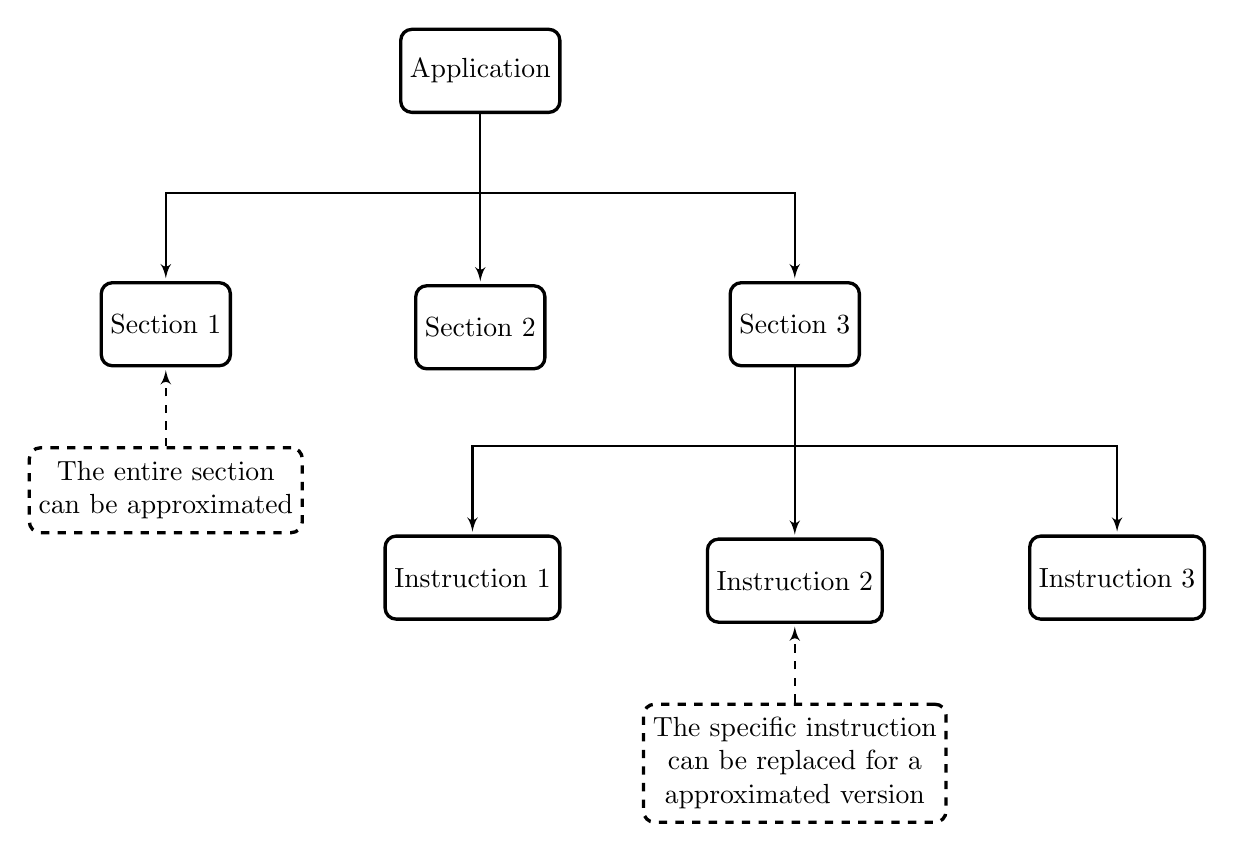
\begin{tikzpicture}[node distance=1cm, auto]  
\tikzset{
    mynode/.style={rectangle,rounded corners,draw=black, very thick, minimum size=3em, text centered},
    myarrow/.style={->, >=latex', shorten >=1pt, thick},
    mylabel/.style={text width=7em, text centered} 
}  
\node[mynode] (manufacturer) {Application};  
\node[mynode, below left =3cm of manufacturer] (section1) {Section 1}; 
\node[mynode, below=2.16cm of manufacturer] (section2) {Section 2};
\node[mynode, below right=3cm of manufacturer] (section3) {Section 3};

\node[mynode, below=1cm of section1, dashed] (comment1) {\makecell{The entire section \\ can be approximated}};

\node[mynode, below left=3cm of section3] (instru1) {Instruction 1};
\node[mynode, below =2.16cm of section3] (instru2) {Instruction 2};
\node[mynode, below right=3cm of section3] (instru3) {Instruction 3};

\node[mynode, below=1cm of instru2, dashed] (comment2) {\makecell{The specific instruction \\ can be replaced for a \\ approximated version}};


\draw[myarrow] (manufacturer.south)  -- ++(0,-1) -|  (section1.north);
\draw[myarrow] (manufacturer.south)   -|  (section2.north);
\draw[myarrow] (manufacturer.south)  -- ++(0,-1) -|  (section3.north); 

\draw[->, >=latex', shorten >=1pt, thick, dashed]  (comment1.north) -|  (section1.south); 

\draw[myarrow] (section3.south)  -- ++(0,-1) -|  (instru1.north);
\draw[myarrow] (section3.south)   -|  (instru2.north);
\draw[myarrow] (section3.south)  -- ++(0,-1) -|  (instru3.north); 
 
 \draw[->, >=latex', shorten >=1pt, thick, dashed]  (comment2.north) -|  (instru2.south); 
 
\end{tikzpicture} 
\medskip
\caption{Expected situation to solve with this project} 
\end{figure}



% Los entregables con consistentes con los objetivos del proyecto y
% con los productos de un proyecto de ingenier�a de software para
% efectos de desarrollo posterior o mantenimiento.
% Los entregables tienen un identificador �nico.
% Los entregables deben incluir:
%	- Documento de Requerimientos
%	- Documento de Dise�o
%	- Plan de pruebas/Resultados de las preubas
%	- Otra documentaci�n relevante: instrucciones de compilaci�n,
% manuales de instalaci�n, manual de usuario etc.
\section{Deliverables and criteria of acceptance}

The expected deliverables are the following:
\begin{table}
\begin{center}
\caption{Deliverables with the corresponding criteria of acceptance}
\begin{tabular}{ |c|c|c| } 
 \hline
Name & Description & Criteria of acceptance \\
 \hline
 Requirement 1.1 & Instances of approximated hardware & [criterio] \\ 
 Requirement 2.1 & Configuration of approximated ASIPs & [criterio] \\ 
 Requirement 3.1 & Data of execution time, area and power & [criterio] \\ %Plan de prueba
 Requirement 3.2 & Comparison and analysis of the obtained results & [criterio] \\ %Plan Prueba
 \hline
\end{tabular}
\label{tab:del}
\end{center}
\end{table}



% Las cuatro �reas analizadas (personal, herramientas, procesos,
% insumos) son analizadas en detalle, identificando los riesgos m�s
% sobresalientes para cada una de esas �reas. Para cada riesgo se
% indica la probabilidad y el impacto para el proyecto.
\section{Risk analysis}
\begin{table}
\begin{center}
\caption{Risk analysis}
\begin{tabular}{ | c | c | c | c | } 
 \hline
 Risk & \makecell{Probability of \\ occurrence} & \makecell{Impact \\ (hours)} & \makecell{Risk exposure \\ (hours)} \\
 \hline
  \makecell{Illness or any special medical condition} & 0.5 & 8 & 4 \\ 
 \makecell{General server errors (missing files, \\ permission restrictions, etc)}   & 0.6 & 24 & 14.4 \\
 \makecell{Delays when acquiring the hardware}   & 0.25 & 8 & 2 \\
 \hline
\end{tabular}
\label{tab:risk}
\end{center}
\end{table}



% Las actividades propuestas son consistentes con los objetivos
% espec�ficos.
% Las estimaciones de esfuerzos son proporcionales con la
% complejidad o el tama�o de las mismas.
% Se asigna un identificador �nico (c�digo) a cada actividad.
\section{Activities and effort budget}

The table \ref{tab:act} takes in consideration a total of 216 engineering hours. 

\begin{table}
\begin{center}
\caption{Activities and effort budget}
\begin{tabular}{ | c | c | c | c | c | } 
 \hline
 ID  &Activity & \makecell{Engineering \\ hours} & \makecell{Risk reserve \\ (hours)} & \makecell{Total \\ (hours)} \\
 \hline
 001 & \makecell{Get to know the software platform} & 24 & 2 & 26 \\
 \hline
\end{tabular}
\label{tab:act}
\end{center}
\end{table}


% El cronograma incluye todas las actividades y las mismas no
% guardan una consistecia l�gica para la construcci�n de los
% entregables.
% Se incluyen hitos para los entregables m�s sobresalientes.
% El nivel de granularidad de las actividades ofrece suficiente detalle.
% Al menos una actividad por semana.
\section{Schedule}

\begin{table}
\begin{center}
\caption{Schedule for the entire project}
\begin{tabular}{ | c | c | c | c | c | c | c | c | c | c | c | c | c | c | c | c | c |} 
 \hline
   & \multicolumn{16}{|c|}{Week} \\
 \hline
 Activity & 1 & 2 & 3 & 4 & 5 & 6 & 7 & 8 & 9 & 10 & 11 & 12 & 13 & 14 & 15 & 16 \\ \hline
 \makecell{Reading the corresponding \\ literature about the \\ project and understanding \\ the general idea of ASIPs}
 & \cellcolor[HTML]{AA0044}  &  &  &  &  &  &  &  &  &  &  &  &  &  &  &  \\ \hline
 \makecell{Execution of the laboratory \\ script to get  to know \\ the software tools like \\ ASIPMeister, Dlxsim, etc}
 & \cellcolor[HTML]{AA0044}  & \cellcolor[HTML]{AA0044}  &  &  &  &  &  &  &  &  &  &  &  &  &  &  \\ \hline
 \makecell{Delivery of the ``Plan Project'' \\ document}
 &  & \cellcolor[HTML]{AA0044}  &  &  &  &  &  &  &  &  &  &  &  &  &  &  \\ \hline
 \makecell{Delivery of the ``Requirements'' \\ document}
 &  &   & \cellcolor[HTML]{AA0044} &  &  &  &  &  &  &  &  &  &  &  &  &  \\ \hline
 \makecell{Delivery of the ``Design'' \\ document}
 &  &   &  & \cellcolor[HTML]{AA0044} &  &  &  &  &  &  &  &  &  &  &  &  \\ \hline
  \makecell{Delivery of the ``Final report'' \\ document}
 &  &   &  &  &  &  &  &  &  &  &  &  &  &  &  & \cellcolor[HTML]{AA0044} \\ \hline
 \end{tabular}
\label{tab:schd}
\end{center}
\end{table}


% Referencias del Background y el Related Work
\bibliographystyle{sty/plainurl}
\bibliography{references}



\end{document}

